\documentclass[11pt, a4paper]{article}
\usepackage{CJKutf8}
\usepackage{amsthm}
\usepackage{ulem}
\usepackage{xcolor}
\usepackage{amsmath}
\usepackage{amssymb}
\usepackage{courier}
\usepackage{geometry}
\usepackage{enumitem}
\usepackage{graphicx}
\usepackage{listings}
\usepackage{algorithm}
\usepackage{algorithmic}
\usepackage{indentfirst}
%\usepackage{float}
\usepackage[perpage,stable]{footmisc} 
\geometry{left=2.7cm, right=2.7cm, top=3cm, bottom=3cm}


\usepackage{graphics}

\usepackage[colorlinks,linkcolor=black,anchorcolor=blue,citecolor=green,
  %	CJKbookmarks=true,
]{hyperref}
\hypersetup{unicode}

\linespread{1.4}
\usepackage{indentfirst}
\setlength{\parindent}{2em}
\hypersetup{hidelinks}

\usepackage{listings}
\lstset{
  numbers=left,
  texcl=true,
  escapechar=`,
  backgroundcolor=\color{lightgray!40!white}, 
  commentstyle=\rm\color{green!30!black},
  basicstyle=\footnotesize\tt,        % the size of the fonts that are used for the code
  breakatwhitespace=false,         % sets if automatic breaks should only happen at whitespace
  breaklines=true,                 % sets automatic line breaking
  captionpos=b,                    % sets the caption-position to bottom
  extendedchars=false,              % lets you use non-ASCII characters; for 8-bits encodings only, does not work with UTF-8
  frame=single,                    % adds a frame around the code
  language=Java,                 % the language of the code
  keywordstyle=\color{blue!70}\bfseries,
  showspaces=false,                % show spaces everywhere adding particular underscores; it overrides 'showstringspaces'
  showstringspaces=false,          % underline spaces within strings only
  showtabs=false,                  % show tabs within strings adding particular underscores
  tabsize=2                       % sets default tabsize to 2 spaces
}

\begin{document}
\begin{CJK*}{UTF8}{gbsn}
  \title{\bf Java程序“快速排序”设计报告}
  \author{马玉坤-1150310618}
  \date{2016年7月20日}
  \maketitle
  \renewcommand{\contentsname}{\textbf{目录}}
  \tableofcontents
  \newpage
  \newpage
  
  \section{题目描述}
  
  快速排序采用的思想是分治思想。
  
  快速排序是找出一个元素(理论上可以随便找一个)作为基准(pivot),然后对数组进行分区操作,使基准左边元素的值都不大于基准值,基准右边的元素值 都不小于基准值,如此作为基准的元素调整到排序后的正确位置。递归快速排序,将其他n-1个元素也调整到排序后的正确位置。最后每个元素都是在排序后的正 确位置,排序完成。所以快速排序算法的核心算法是分区操作,即如何调整基准的位置以及调整返回基准的最终位置以便分治递归。

  使用Java语言编写一个简单的快速排序程序,能够将一个序列按照递增序排序。

  \section{总体设计思想}
  
  使用quickSort函数对数组的一个连续子序列$a[l..r]$进行排序。在quickSort中,找到基准元素$x = a[p]$(p为$[l,r]$中的一个随机数),然后按照基准元素,将$a[l..r]$分为两个部分,左半部分小于$x$,右半部分大于等于$x$。设x的位置为$mid$,递归调用quickSort,对区间$[l,mid-1]$和$[mid+1,r]$进行排序。

  \section{详细设计}

  \subsection{quickSort函数}
  \subsubsection{函数原型}

  \begin{lstlisting}
    static void quickSort(int l, int r, int[] a);
  \end{lstlisting}

  \subsubsection{作用}

  将$a$数组的$l..r$区间进行排序。

  \subsubsection{函数体}

  
  \begin{lstlisting}
  static void quickSort(int l, int r, int[] a) {
    if (l < r) {
      int mid = partition(l, r, a);
      
      // 递归排序左半部分
      quickSort(l, mid - 1, a);
      
      // 递归排序右半部分
      quickSort(mid + 1, r, a);  
    }
  }

  \end{lstlisting}

  %%%%-------------------partition------------------%%%%
  \subsection{partition函数}
  
  \subsubsection{函数原型}

  \begin{lstlisting}
    static int partition(int l, int r, int[] a);
  \end{lstlisting}

  \subsubsection{作用}

  随机获取$a[l..r]$中一个基准元素,然后按照基准元素的大小将$a[l..r]$分为$a[l..mid-1]$和$a[mid+1..r]$两部分,并返回mid。

  \subsubsection{函数体}
  \begin{lstlisting}
  static int partition(int l, int r, int[] a) {
    
    // 在区间[l,r]中获得一个随机的位置p
    int p = l + rnd.nextInt(r-l);

    // 交换a[l]和a[p]
    int tmp = a[l];
    a[l] = a[p];
    a[p] = tmp;

    // 将a[l]设为基准(pivot)
    int x = a[l];
    
    while (l < r) {

      // 从右边找到第一个小于基准的元素,并将其插入到自由位置(l)中
      while (l < r && a[r] >= x)
        r--;
      if (l < r) {
        a[l] = a[r];
        l++;
      }

      // 从左边找到第一个大于等于基准的元素,并将其插入到自由位置(r)中
      while (l < r && a[l] < x)
        l++;
      if (l < r) {
        a[r] = a[l];
        r--;
      }
    }

    // 将基准元素重新插入到序列中
    a[l] = x;
    return l;
  }
  \end{lstlisting}
  
  
  \section{具体实现}
  \begin{lstlisting}
import java.util.*;

public class quicksort {
  
  static void shuffleArray(int[] a)
  {
    /**
     * `该函数的作用是将a数组随机打乱`
     */
    Random rnd = new Random();
    for (int i = a.length - 1; i > 0; i--)
    {
      int index = rnd.nextInt(i + 1);
      int tmp = a[index];
      a[index] = a[i];
      a[i] = tmp;
    }
  }
  
  static Random rnd = new Random();
  static int partition(int l, int r, int[] a) {
    
    // 在区间[l,r]中获得一个随机的位置p
    int p = l + rnd.nextInt(r-l);

    // 交换a[l]和a[p]
    int tmp = a[l];
    a[l] = a[p];
    a[p] = tmp;

    // 将a[l]设为基准(pivot)
    int x = a[l];
    
    while (l < r) {

      // 从右边找到第一个小于基准的元素,并将其插入到自由位置(l)中
      while (l < r && a[r] >= x)
        r--;
      if (l < r) {
        a[l] = a[r];
        l++;
      }

      // 从左边找到第一个大于等于基准的元素,并将其插入到自由位置(r)中
      while (l < r && a[l] < x)
        l++;
      if (l < r) {
        a[r] = a[l];
        r--;
      }
    }

    // 将基准元素重新插入到序列中
    a[l] = x;
    return l;
  }
  
  static void quickSort(int l, int r, int[] a) {
    if (l < r) {
      int mid = partition(l, r, a);
      
      // 递归排序左半部分
      quickSort(l, mid - 1, a);
      
      // 递归排序右半部分
      quickSort(mid + 1, r, a);  
    }
  }
  
  public static void main(String Args[]) {
    
    // 生成一个0..99999的随机排列
    int[] a= new int[100000];
    for (int i = 0; i < a.length; i++)
      a[i] = i;
    shuffleArray(a);

    // 进行快速排序
    quickSort(0, a.length-1, a);

    // 检查排序结果
    boolean flag = true;
    for (int i = 0; i < a.length - 1; i++) {
      if (a[i] != i) {
        System.out.println("ERROR");
        flag = false;
      }
    }
    if (flag)
      System.out.println("FINISHED");
  }
}

  \end{lstlisting}

  \section{运行结果}

  \begin{center}
    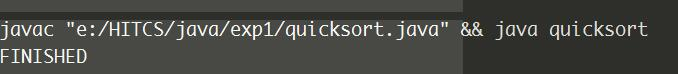
\includegraphics[width=5in]{result.jpg}
  \end{center}

  \newpage  
\end{CJK*}
\end{document}
